\documentclass[11pt,oneside]{book}

\usepackage{array}
\usepackage[printonlyused, withpage]{acronym}
\usepackage[ruled, lined, linesnumbered, noend ]{algorithm2e}
\usepackage{amsmath, amssymb, amsthm}
\usepackage[toc,page]{appendix}
\usepackage{caption}
\usepackage{color}
\usepackage[english]{babel} 
\usepackage{epsfig}
\usepackage{fancybox}
\usepackage{float}
\usepackage[acronym, nomain]{glossaries}
\usepackage{graphicx}
\usepackage{listings}
\usepackage{microtype}
\usepackage{moreverb}
\usepackage{multirow}
\usepackage{pdfpages}
\usepackage{subfigure}
\usepackage{todonotes}
\usepackage{url}

\usepackage[utf8]{inputenc}
\usepackage[final, bookmarks, breaklinks, colorlinks, allcolors=black]{hyperref}
\usepackage[autostyle=true]{csquotes} % Required to generate language-dependent quotes in the bibliography
\usepackage[sorting=none]{biblatex} % Use the bibtex backend with the authoryear citation style (which resembles APA)
\addbibresource{sections/bibliography.bib} % The filename of the bibliography

\newtheorem{problem}{Problem}

\theoremstyle{definition}
\newtheorem{definition}{Definition}

\definecolor{mygreen}{rgb}{0,0.6,0}
\definecolor{mygray}{rgb}{0.5,0.5,0.5}
\definecolor{mymauve}{rgb}{0.58,0,0.82}
\lstset{ %
	backgroundcolor=\color{white},   % choose the background color; you must add \usepackage{color} or \usepackage{xcolor}; should come as last argument
	basicstyle=\footnotesize,        % the size of the fonts that are used for the code
	breakatwhitespace=false,         % sets if automatic breaks should only happen at whitespace
	breaklines=true,                 % sets automatic line breaking
	captionpos=b,                    % sets the caption-position to bottom
	commentstyle=\color{mygreen},    % comment style
	deletekeywords={...},            % if you want to delete keywords from the given language
	escapeinside={\%*}{*)},          % if you want to add LaTeX within your code
	extendedchars=true,              % lets you use non-ASCII characters; for 8-bits encodings only, does not work with UTF-8
	frame=single,
	keepspaces=true,                 % keeps spaces in text, useful for keeping indentation of code (possibly needs columns=flexible)
	keywordstyle=\color{blue},       % keyword style
	morekeywords={*,...},            % if you want to add more keywords to the set
	numbers=left,                    % where to put the line-numbers; possible values are (none, left, right)
	numberstyle=\tiny\color{mygray}, % the style that is used for the line-numbers
	rulecolor=\color{black},         % if not set, the frame-color may be changed on line-breaks within not-black text (e.g. comments (green here))
	showspaces=false,                % show spaces everywhere adding particular underscores; it overrides 'showstringspaces'
	showstringspaces=false,          % underline spaces within strings only
	showtabs=false,                  % show tabs within strings adding particular underscores
	stringstyle=\color{mymauve},     % string literal style
	tabsize=2,	                     % sets default tabsize to 2 spaces
	title=\lstname                   % show the filename of files included with \lstinputlisting; also try caption instead of title
}

\lstdefinelanguage{FLY} {
  morestring=[b]",
  morecomment=[l]{//},
  morecomment=[s]{/}{/},
  identifierstyle=\color{black},
  keywordstyle=\color{javapurple},
  morekeywords={func,var,while, if, then, else,for, in, println, fly ,on,thenall,as,then,require,native}% list your attributes here
}

\lstset {
    language=FLY,
    basicstyle=\ttfamily\scriptsize,    
    keywordstyle=\color{javapurple}\bfseries,
    stringstyle=\color{javared},
    commentstyle=\color{javagreen},
    morecomment=[s][\color{javadocblue}]{/*}{/},
    numbers=left,
    numberstyle=\tiny\color{black},
    stepnumber=1,
    numbersep=10pt,
    tabsize=4,
    showspaces=false,
    showstringspaces=false
}


\begin{document}
    \begin{titlepage}
        \begin{center}
            
\epsfig{file=figures/logo_standard.jpg,width=2.5truecm}\\[0.2truecm]
            {\Large Universit\`a degli Studi di Salerno}\\[0.2truecm]
            {\large Dipartimento di Informatica}\\
            \hrulefill
            \vfill
            {\large Tesi di Laurea di II livello in }\\[0.2truecm]
            {\Large Informatica}\\
            \vfill\vfill
            {\Huge An Empirical Assessment on the Effectiveness of Test-Driven Development Techniques for Embedded Systems}
            \vfill\vfill
            
            
            {\bf Relators} \hfill {\bf Candidate}\ \ \\
            Giuseppe Scanniello \hfill Michelangelo Esposito\\
            Simone Romano \hfill \ \ \\
            
            \vfill
            \hrulefill 
            
            Academic Year 2021-2022
        
        \end{center}
    \end{titlepage}


    \pagenumbering{roman}
    \chapter*{Abstract}
    Lorem ipsum dolor sit amet, consectetur adipiscing elit, sed do eiusmod tempor incididunt ut labore et dolore magna aliqua. Ut enim ad minim veniam, quis nostrud exercitation ullamco laboris nisi ut aliquip ex ea commodo consequat. Duis aute irure dolor in reprehenderit in voluptate velit esse cillum dolore eu fugiat nulla pariatur. Excepteur sint occaecat cupidatat non proident, sunt in culpa qui officia deserunt mollit anim id est laborum.
    
    \tableofcontents
    \pagestyle{plain}

    \thispagestyle{empty}
\listoffigures

    \chapter*{List of Acronyms and Abbreviations}
    \DeclareAcronym{ga}{
  short = GA,
  long = Genetic Algorithm,
}

\DeclareAcronym{ai}{
  short = AI,
  long = Artificial Intelligence,
}

\DeclareAcronym{ws}{
  short = WS,
  long = Whole Suite,
}

%%% algorithms %%%
\DeclareAcronym{nsga-ii}{
  short = NSGA-II,
  long = Non-dominated Sorting Genetic Algorithm-II,
}

\DeclareAcronym{mosa}{
  short = MOSA,
  long = ,
}

\DeclareAcronym{dynamosa}{
  short = DynaMOSA,
  long = ,
}

%%% IOt %%%
\DeclareAcronym{iot}{
  short = IoT,
  long = Intenet of Things,
}

\DeclareAcronym{es}{
  short = ES,
  long = Embedded System,
}

\DeclareAcronym{cps}{
  short = ES,
  long = Embedded System,
}

    \chapter{Introduction}
    \setcounter{page}{1} 	% must only follow the first chapter
    \pagenumbering{arabic}	% must only follow the first chapter
    A computer hardware and software combination created for a particular purpose is an Embedded System (\es). In many cases, \ess operate as part of a bigger system (\eg  agricultural and processing sector equipment, automobiles, medical equipment, airplanes, and so on) and within tight resource constrains (\eg small battery, limited memory and CPU speed, and so on).
The global \ess market is expected to witness notable growth. A recent report evaluated the  global \ess market 89.1 billion dollars in 2021, and this market is projected to reach 163.2 billion dollars by 2031; with a compound annual growth rate of  6.5\%~ \cite{ESSTR2022}. This growth is mostly related to  an increase in the demand for advanced driver-assistance system (in electric and hybrid vehicles) and in the number of \ess-related research and development projects.  


Test-Driven Development (\tdd) is an incremental approach to software development in which a developer repeats a short development cycle made up of three phases: \textit{red}, \textit{green}, and \textit{blue/refactor} \cite{TDDByExample}. During the red phase, the developer writes a unit test for a small chunk of a functionality not yet implemented and watches the test fail. In the green phase, the developer implements the chunk of functionalities as quickly as possible and watches all the unit tests pass. During the refactoring phase, the developer changes the internal structure of the code while paying attention to keep the functionality intact—accordingly, all unit tests should pass. TDD has been conceived to develop “regular” software, and it is claimed to improve software quality as well as developers' productivity \cite{DBLP:reference/se/ErdogmusMJ10}. \ess have all the same challenges of non-embedded systems (\noess), such as poor quality, but add challenges of their own [6]. 
For example, one of the most cited differences between embedded and \noess is that embedded code depends on the hardware. While in principle, there is no difference between a dependency on a hardware device and one on a \noess \cite{TDDEC}, dealing with hardware introduces a whole new set of variables to consider during development. Furthermore, the limited resources on which an \es usually operates may make it extremely difficult to properly test the system in its entirety. 
Over the years, a huge amount of empirical investigations has been conducted to study the claimed effects of TDD on the development of \noess (\eg, \cite{DBLP:journals/software/KaracT18}). So far no investigations have been conducted to assess possible benefits concerned the application of TDD on the development of \ess although some authors, like Greening \cite{TDDEC}, believes that embedded developers can benefit from the application of TDD in the development of \ess.

In this work of thesis, we investigate the following primary research question (RQ):
\\ \ \\
\noindent \textbf{RQ.} Does the use of \tdd affect the development of \ess?	
\\ \ \\
To answer this RQ, we present the results of a controlled (baseline) experiment and its replication to study the application of \tdd on the implementation of \ess. The participants were final year Master Students in Computer Science enrolled to an \es course at the University of Salerno. The goal of these experiments is to increase our body of knowledge on the benefit (if any) related to the application of \tdd in the context of the development of \ess. To that end, we compare \tdd with respect to a more traditional, test-last, development practice, where test cases are written after the production code. From here onwards, we refer to this traditional way of coding as \notdd. Whichever the used approach (\tdd and \notdd), the participants in the implementation of an \es where asked to use a mock to model and confirm the interactions between a device driver and the hardware. The mocked implementation would intercept commands to and from the device simulating a given usage scenario. In the replication experiment, the participants had to implement a more complex \es and had also to replace the mocks with real hardware components (a number of sensors and actuators) before deploying the \es on the actual hardware platform they had mocked up to that point. The logic of the \es was deployed on Raspberry Pi model 3 and the developed test cases were executed in the real environment. Variations in the replicated experiments (task and the experimental procedure) were introduced to validate the results of the baseline experiment and to generalize these results to a more real setting. The results obtained by an aggregated analysis of the data from both the experiments suggest that there are no significant differences between \tdd and \notdd on: productivity, number of written tests, a..., respectively. On the other hand, we observed a significant difference on: ... When analyzing experiments individually, we observed that ...

As for the following thesis structure, it is made up of five chapters:
The first two act as the foundational knowledge concepts that provide a general overview on the main topics surrounding \tdd and \es.
More in detail, chapter one contains an overview on the software testing process, analyzing the main approaches, with a focus on \tdd. Chapter two will provide information on the general \ess concepts, enabling technologies and implementation challenges, before discussing the techniques for testing such systems.
In chapter three, we conduct a review of the literature by examining the most relevant previous empirical studies on the application of \tdd and the current testing methodologies for \es.
Chapter four will contain the detail explanation of our approach for the definition of the two experimental studies, the analysis of the results, and our answers to the research questions.
Finally, chapter five will provide the conclusions to the thesis, along with a discussion on the possible ramification the research could manifest when moving forward in the analysis of \tdd for \es development.

    \chapter{Test Driven Development}
    \section{Overview on software testing}
Software testing is an essential part of the development process of a system, as it helps to ensure that a piece of software is reliable and performs as intended; it can be defined as the process of finding differences between the expected behavior specified by system's requirements and models, and the observed behavior of the implemented software. Unfortunately, it is impossible to completely test a nontrivial system. First, testing is not decidable. Second, testing must be performed under time and budget constraints \cite{OOSE}, therefore developers often compromise on testing activities by identifying only a critical subset of features to be tested.

There are many approaches to software testing, including unit testing, integration testing, system testing, as well as performance, penetration and acceptance testing. Each of these approaches has its own specific goals and methods, and they are often used in combination to ensure that a software product is thoroughly tested and conform to its specification.
\begin{itemize}
    \item \textbf{Unit Testing} is a method of testing individual units or components of a software product in isolation; its goal is to verify that each unit of code is working correctly and meets the specified requirements. Unit tests are typically written by the developers who wrote the code, and they are run automatically as part of the build process. Techniques also exist to generate input configuration for unit test automatically, by searching amongst the input space for the tests.
    \item \textbf{Integration Testing} is a method of testing how different units or components of a software product work together. The goal of integration testing is to ensure that the different parts of the system are integrated correctly and that they function as expected when combined. Integration tests are typically more complex than unit tests, as they involve multiple units of code working together.
    \item \textbf{System Testing} is a method of testing a complete software product in a simulated or real-world environment. The goal of system testing is to ensure that the software meets the specified requirements and performs as expected when running in a real-world environment. System tests may involve testing the software on different hardware or operating systems, or with different data inputs and configurations.
    \item \textbf{Acceptance Testing} is a method of testing a software product to ensure that it meets the needs and expectations of the end user. The goal of acceptance testing is to verify that the software is fit for its intended purpose and that it meets the requirements of the user. Acceptance tests are often written by the end user or a representative of the end user, and they may involve testing the software in a real-world environment
\end{itemize}


\subsection{Software Development Lifecycle}
Before discussing how testing activities are performed in more detail, it is essential to introduced how testing is integrated in the development process. The term Software Development Lifecycle, SDLC, refers to the entire process of developing and maintaining software systems. It includes the following phases:

\begin{figure}[h]
    \centering
    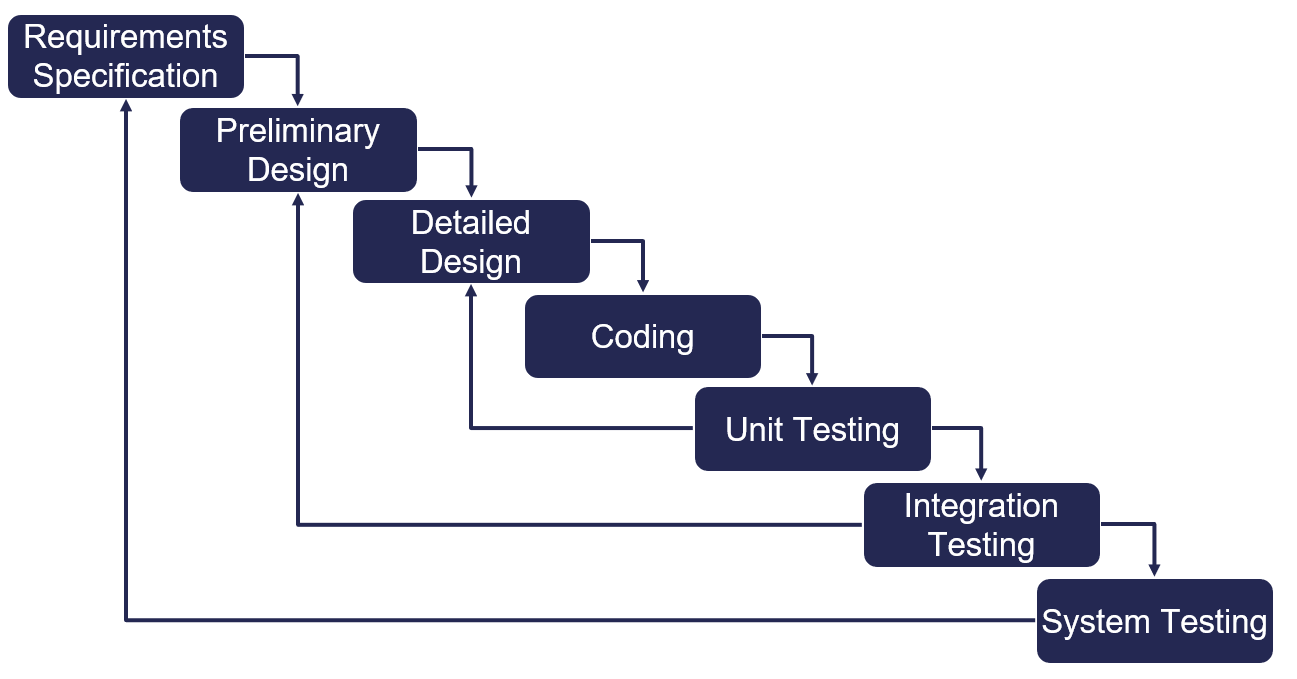
\includegraphics[width=\linewidth]{figures/waterfall_model.png}
    \caption{The Waterfall model}
    \label{waterfall_model}
\end{figure}

The main weakness of the Waterfall model is the very long feedback cycle between requirements specification and system testing; during this phase, the client is absent and there is no deliverable product before the end of the process

Modern software development strays away from non-incremental models, as today's applications are continuously evolving and adapting; instead

\begin{figure}[h]
    \centering
    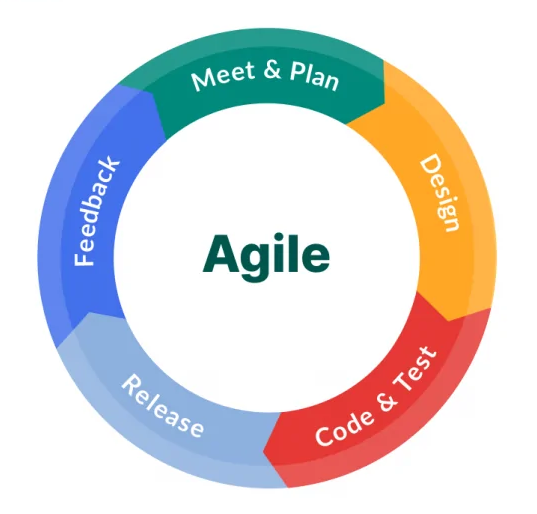
\includegraphics[width=\linewidth]{figures/agile_model.jpg}
    \caption{The Agile model}
    \label{agile_model}
\end{figure}



\section{Test Driven Development}

\subsection{Overview}
The concept of Test Driven Development (TDD) was firstly introduced in 2003 by Kent Back in the book "Test Driven Development By Example" \cite{TDDByExample}. While there is no formal definition of the process, as the author states, the goal is to "write clean code that works".
Compared to traditional SDL processes, TDD is an extremely short, incremental, and repetitive process, and is related to \textbf{test-first programming} concepts in extreme programming; this advocates for frequent updates/releases for the software, in short cycles, while encouraging code reviews, unit testing and incremental addition of features.


At its core, TDD is made up of three iterative phases: "Red", "Green" and "Blue" (or "Refactor"):
\begin{itemize}
    \item In the "\textbf{Red}" phase, a test case is written for the chunk of functionality to be implemented; since the corresponding logic does not exist yet, the test will obviously fail, often not even compiling.
    \item In the "\textbf{Green}" phase, only the code that is strictly required to make the test pass is written.
    \item Finally, in the "\textbf{Blue}" phase, the implemented code, as well as the respective test cases, is refactored and improved. It is important to perform regression testing after the refactoring to ensure that the changes didn't result in any unexpected behaviors in other components.
\end{itemize}
Each new unit of code requires a repetition of this cycle \cite{GuidelinesTDD}.

The figure below provides a representation of the TDD cycle:
\begin{figure}[h]
    \centering
    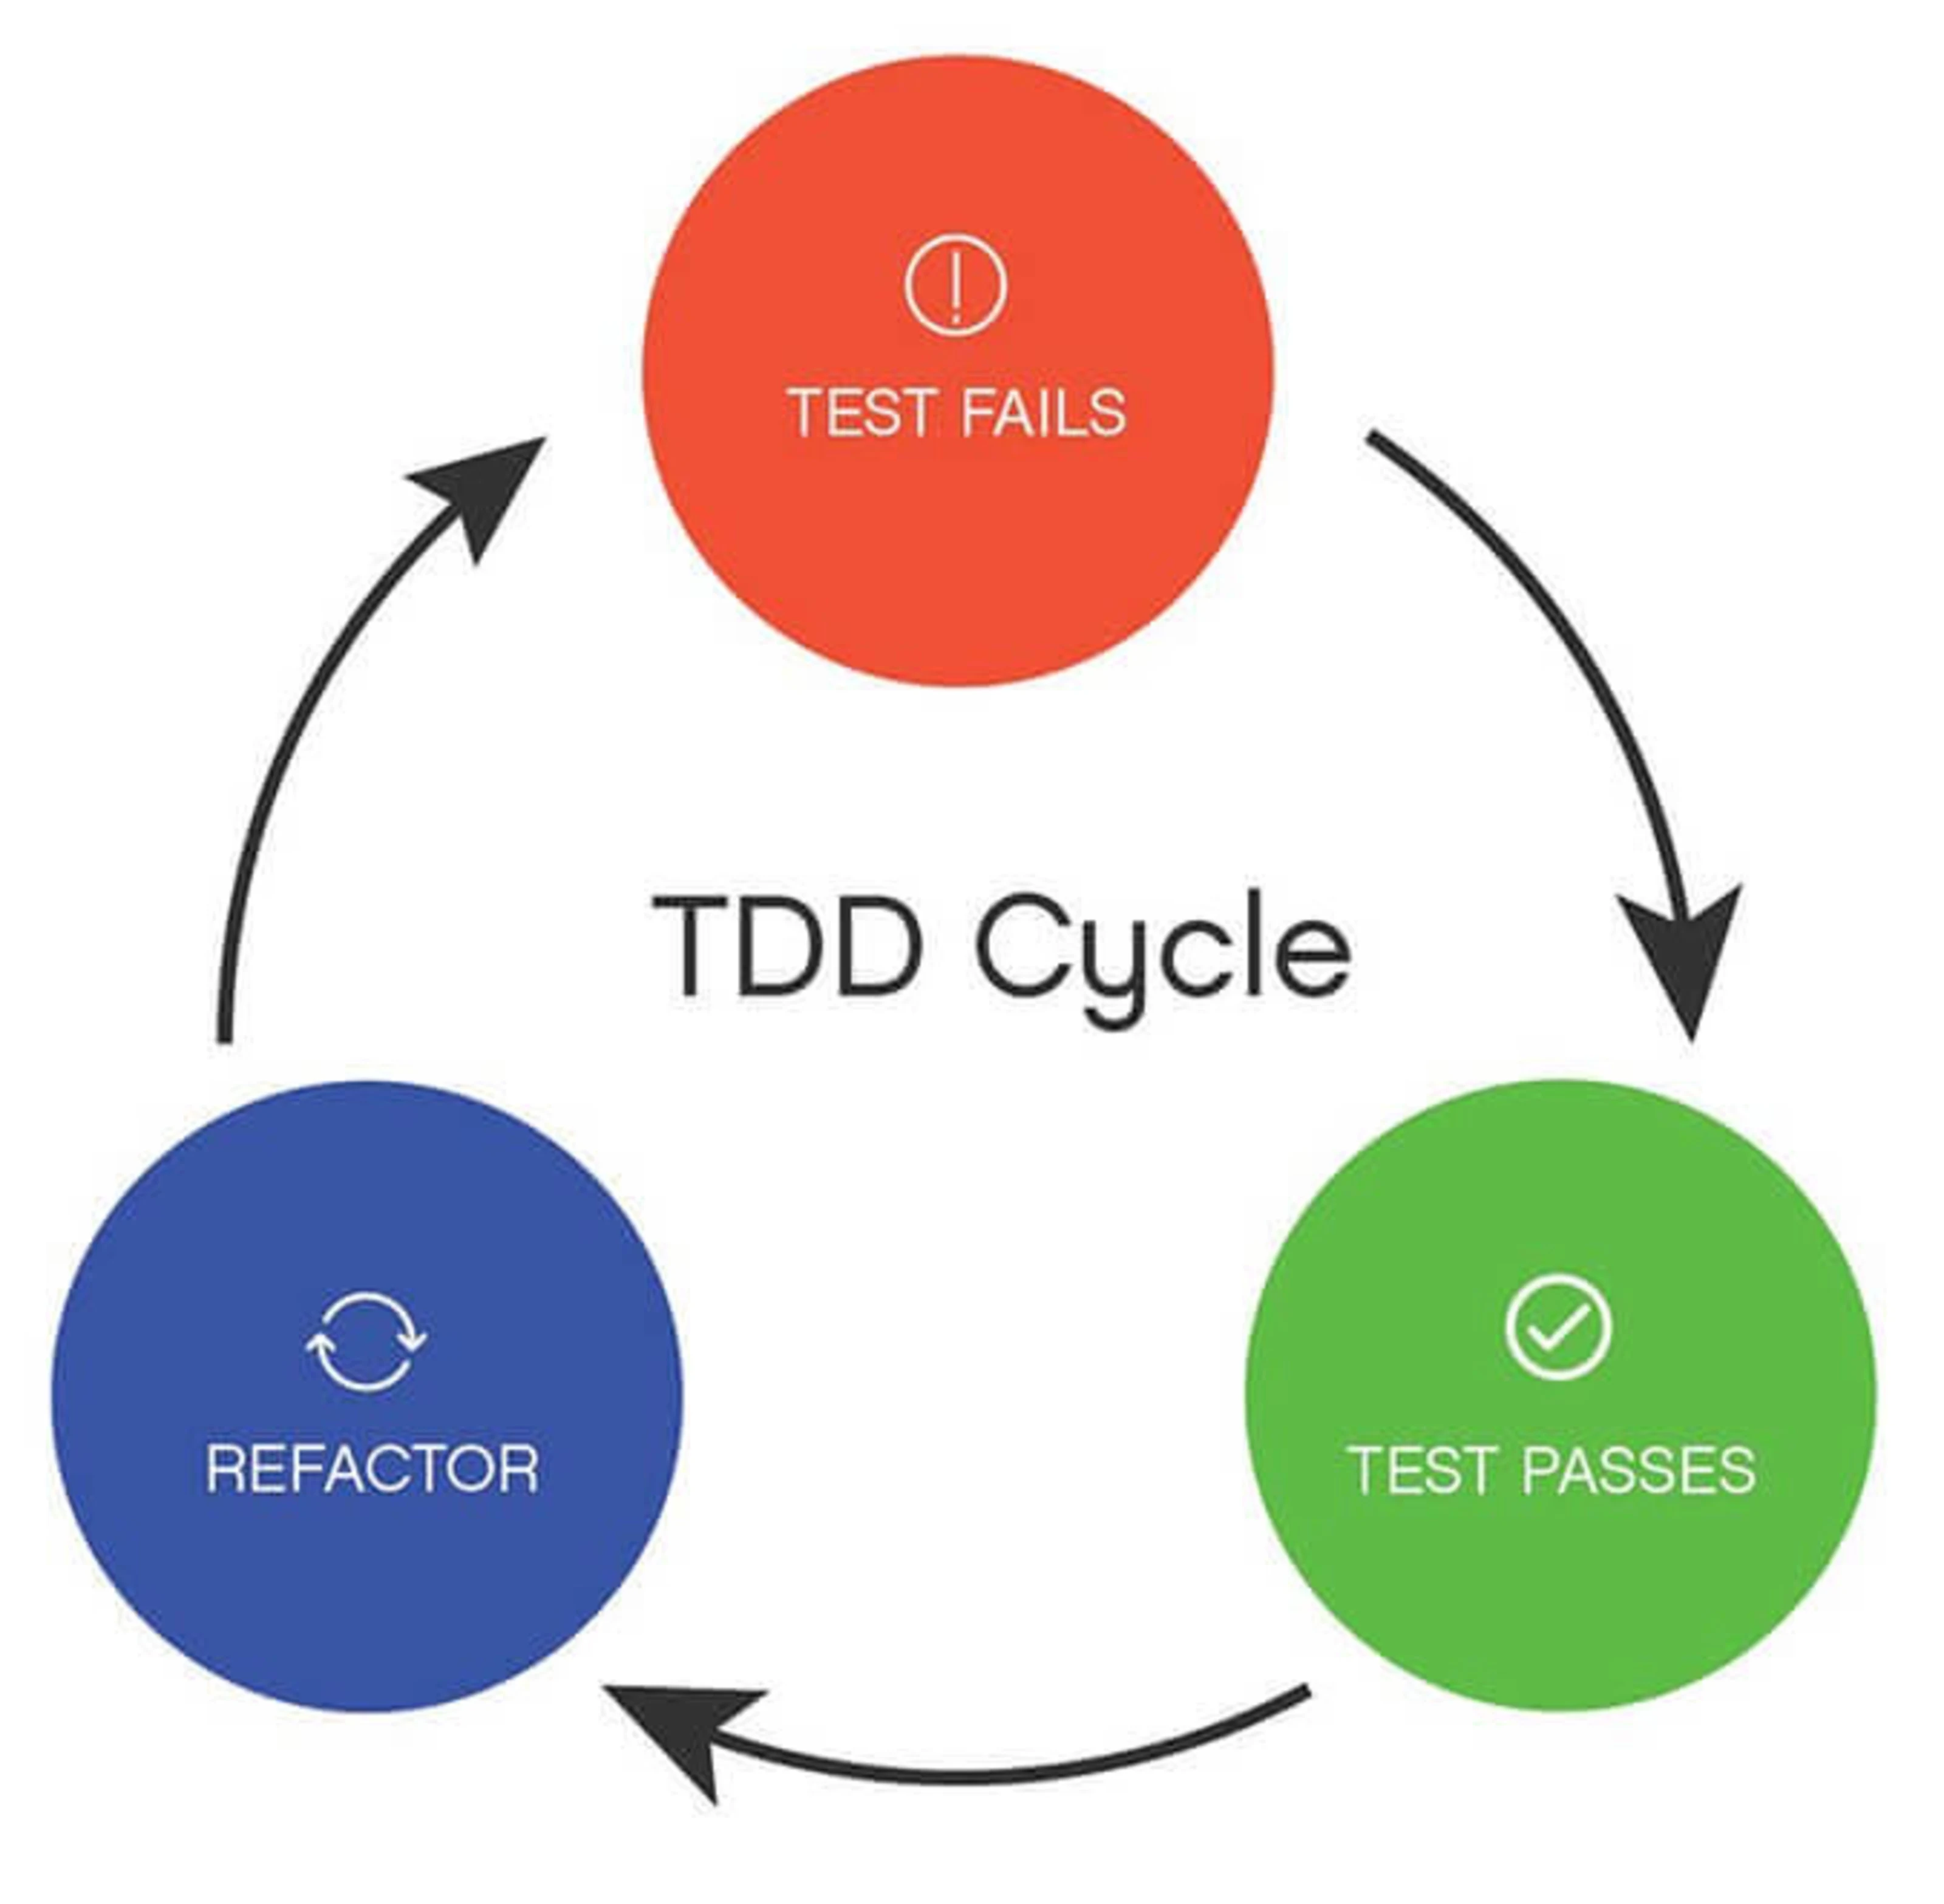
\includegraphics[width=\linewidth]{figures/tdd_cycle.jpg}
    \caption{The Test Driven Development cycle}
    \label{fig}
\end{figure}

As previously stated, each TDD iteration should be extremely short, usually spanning from 10 to 15 minutes at most; this is possible thanks to a meticulous decomposition of the system's requirements into a set of \textbf{User Stories}, each detailing a small chunk of a functionality specified in the requirements. These stories can then be prioritized and implemented iteratively.

User stories can vary in granularity: when using a fine-grained structure when describing the task, this can be broken up into a set of sub-tasks, each corresponding to a small feature; on the other hand, with coarser-grained tasks, this division is less pronounced \cite{DBLP:journals/tse/KaracTJ21}. Even when the same task is considered, the outcome of the TDD process will change depending on the level of granularity employed when describing it; there is no overall right or wrong approach, rather it is something that comes from the experience of the developer to break tasks into small work items \cite{DBLP:journals/tse/KaracTJ21}.

The general mantra of TDD revolves around the "Make it green, then make it clean" motto

\subsection{TDD advantages}
The employment of TDD can result in a series of benefits during the development process, such as:
\begin{itemize}
    \item \textbf{Regression testing}: by incrementally building a test suite as the different iterations of TDD are performed, we ensure that the system  
    \item \textbf{Very high code coverage}: coverage is a metric used to determine how much of the code is being tested; it can be expressed according to different criteria such as statement coverage, i.e., how many statements in the code are reached by the test cases, branch coverage, i.e., how many conditional branches are executed during testing, or function coverage, i.e., how many functions are executed when running the test suite. While different coverage criteria result in different benefits, by employing TDD we ensure that any segment of code written has at least one associated test case.
    \item \textbf{Improved code quality}: as we are specifically writing code to pass the tests in place, and refactoring it after the "Green" phase, we ensure that the code is cleaner and overall more optimized, without any extra pieces of functionalities that may not be needed. 
    \item \textbf{Improved code readability and documentation}: test act as documentation...
    \item \textbf{Simplified debugging and early fault detection}: Whenever a test fails it becomes obvious which component has caused the fault: by adopting this incremental approach and performing regression testing, if a test fail we will be certain that the newly written code will be responsible. For this reason, faults are detected extremely early during the testing process, rather than potentially remaining hidden until the whole test suite has been built and executed.
\end{itemize}




    \chapter{Testing Embedded Systems}
    \section{Overview on Embedded Systems}
Embedded Systems (ES) can be defined as a combination of hardware components and software systems that seamlessly work together to achieve a specific purpose; such systems can be dynamically programmed or have a fixed functionality set, and are often engineered to achieve their goal within a larger system. They are often found in devices that we use on a daily basis, such as cell phones, traffic lights, and appliances. Here, these systems are responsible for controlling the functions of the device, and they are often required to work continuously without the need for human intervention.

Often enough, ES must operate in a stand-alone manner: many of these systems are used in environments where there is no access to a network or the internet, so the ability to function independently is essential; this requires the use of embedded software, which is specifically designed to run on the limited hardware of the system.

In recent years, such system have seen a steep surge in popularity, and have driven innovation forward in their respective areas of deployment: everywhere, spanning from the agricultural field, to the medical and energy ones, ES of various size and complexity are employed, especially in areas where human intervention is impractical or straight up impossible.
As the demand for more advanced and sophisticated devices continues to increase, the role of ES will only become more prominent.

There are many different types of embedded systems, including microcontrollers, digital signal processors (DSPs), and field-programmable gate arrays (FPGAs). Each of these types of systems has its own unique characteristics and is suited to different types of applications.

General purpose hardware, Arduino, Raspberry, etc...



\section{Enabling technologies}
One of the key enabling technologies for ES is their microcontroller, which is a small, single-chip computer that is used to manage the functions of the larger system. Microcontrollers are often used in embedded systems because they are cheap, low-power. While some applications require their own custom-made microcontroller and hardware, there are a variety of  general purpose boards that are far easier to program and can also be customized for a variety of applications, which makes them highly versatile.

One type of general-purpose microcontroller that is commonly used for ES development, as well as many other IoT applications, is the Arduino; it is an open-source platform that is based on the Atmel AVR microcontroller. It is widely used in hobbyist and educational projects because of its simplicity and low cost. Another popular general-purpose microcontroller platform is the Raspberry Pi, which is a small single-board computer that is based on the ARM architecture, which is also what many mobile processors are based on.

In addition to these general-purpose microcontrollers, there are also many proprietary microcontrollers that are designed for specific applications: these microcontrollers are often customized for a particular task and may not be easily programmable by the user. Some examples of proprietary microcontrollers include the Microchip PIC and the Texas Instruments MSP430. These chips are often used in industrial and commercial applications where a high level of performance and reliability is required. They may also be used in applications where security is a concern, as the design of these microcontrollers may be kept confidential to protect against tampering or reverse engineering.

Overall, the choice of microcontroller for an ES will depend on the specific requirements of the application. General-purpose microcontrollers such as Arduino and Raspberry Pi may be suitable for hobbyist or educational projects, while proprietary microcontrollers may be better suited for industrial or commercial applications where performance and reliability are critical.


Software-wise, more complex system can be equipped with their own \textbf{Embedded Operating System}, or more specifically, their \textbf{Real-Time Operating System} (RTOS); these are specialized operating systems that are designed to provide a predictable response time to events, even when there are many tasks running concurrently. RTOS are essential for embedded systems that require fast and reliable performance, such as in aircraft control systems or medical devices.

Often, multiple devices are deployed as part of the same larger system and must be able to efficiently communicate between one another to achieve their purpose; therefore, it is essential for ES to ... a robust suite of protocols.
As always, determine which protocol to employ depends on the constraints the system is dealing with, such as being limited to a low power consumption or being required to maintain a low-latency communication.

Zigbee is a wireless communication protocol specifically designed and built for low-power, low-data-rate applications \cite{Zigbee}; it is often used in sensors and other devices that need to communicate over short distances, such as in home automation systems or industrial control systems. One of its key advantages is its very low power consumption, which makes it so ZigBee is one of the most well-suited protocols for use in devices that need to operate for long periods of time without access to a power source (i.e., a quite substantial subset of ESs).

Bluetooth is another wireless protocol that is commonly used in embedded systems which was designed for medium-range communication and is most commonly used to connect devices such as phones, tablets, and laptops to other devices, such as speakers, keyboards, or headphones. Bluetooth is a widely supported standard and is often used in applications where compatibility with a range of different devices is important; furthermore, with its low-energy variant, Bluetooth can help further optimize power consumption in devices that require it.

SigFox on the other hand, is a low-power, wide-area (LPWA) communication protocol that is designed for Internet of Things (IoT) applications; it is used to transmit small amounts of data over long distances, making it well-suited for use in remote monitoring systems or other applications where conventional communication methods are not practical.

For network communications, IP, and it's low energy version 6LoWPAN, are widely used protocols. It is used to transmit data between devices and is a key component of the internet. IP is often used in embedded systems that need to communicate with other devices or with the internet, such as in smart home systems or industrial control systems.

Overall, each of these protocols has its own strengths and is well-suited for different types of applications. Zigbee is ideal for low-power, low-data-rate applications, while Bluetooth is well-suited for medium-range communication. Sigfox is ideal for long-range communication in IoT applications, and IP is widely used for communication over networks.



\section{Design}
From a design and development point of view, working with ES can be complex, as it involves a wide range of skills and disciplines, including computer science, electrical engineering, and mechanical engineering. It is often necessary to work closely with other team members, including hardware and software designers, to ensure that the system meets all the requirements.

Failures in ES should always be evident and identifiable quickly (a heart monitor should not fail quietly \cite{MakingEmbeddedSystems}). Given the high criticality of such systems, ensuring their dependability over the course of their lifespan is essential; ES can be deployed in extreme conditions (i.e., weather monitoring in extreme locations of the planet, devices inside the human body, or \dots), where maintenance operations cannot be performed regularly,  and high availability is expected. 

The dependability of a system can be expressed in terms of:
\begin{itemize}
    \item \textbf{System maintainability}: the extent to which a system can be adapted/modified to accommodate new change requests. As ES becomes more complex and feature-rich, it is becoming increasingly important to design them with maintainability in mind. This includes designing systems that are easy to update and repair, as well as ensuring that they can be easily replaced if necessary.
    \item \textbf{System reliability}: the extent to which a system is reliable with respect to the expected behavior.
    \item \textbf{System availability}: the extent to which a system remains available for its users.
    \item \textbf{System security}: the extent to which a system can keep data of its users safe and ensures the safety of their users.
\end{itemize}

These dependability attributes cannot be considered individually, as there are strongly interconnected; for instance, safe system operations depend on the system being available and operating reliably in its lifespan. Furthermore, an ES can be unreliable due to its data being corrupted by an external attack or due to poor implementation. As a result of particular care should be applied in the design of these systems, especially \dots 


In conclusion, ES are specialized computer systems that are designed to perform a specific task within a larger system; they are able to perform real-time processing and operate in a stand-alone manner, but they also face the challenge of limited resources and power. Despite this, the use of ES has grown significantly, and they are now found in a wide variety of applications.



\section {Challenges}
An important, and often critical, aspect of ES, which defines the greatest challenges when engineering them, is the limited quantity resources available: these systems often have very small amounts of memory and processing power, so it is important to carefully design the software to make the most efficient use of them. This can involve using specialized programming languages and techniques, such as real-time operating systems and low-level hardware access. Furthermore, many such systems may be powered by using a battery, and thus the hardware they are equipped with, often purpose built, must be highly efficient in its operations. Furthermore, from the software point-of-view, it is essential that the system operates deterministically and with real-time constrains.

Another notable challenge is the requirement of some systems to perform real-time processing tasks. This means that they must be able to process data and provide a response within a specific time frame. For example, an embedded system in a car might be responsible for controlling the engine and transmission; it must be able to process data from sensors and make decisions about how to control the engine and transmission in real-time, as the car is being driven.

In addition to the technical challenges, there are also many non-technical factors that must be considered when developing embedded systems. For example, the system must be able to operate within the physical constraints of the device it is being used in, and it must be able to withstand the environmental conditions in which it will be used.



\section{Testing Embedded Systems}
Testing ES poses a series of challenges compared to traditional testing: first of all, in the case of ES that are highly integrated with a physical environment (such as with CPSs), replicating the exact conditions in which the hardware will be deployed may be challenging. Secondly, field-testing of these systems can be unfeasible to dangerous or impractical environmental conditions (i.e., a nuclear power plant, a deep-ocean station, or the human body). Furthermore, given the absence of a user interface in most cases, testing such systems can be particularly challenging, given the lack of immediate feedback. Finally, the testing of time-critical systems has to validate the correct timing behavior which means that testing the functional behavior alone is not sufficient; similarly, system with tight hardware constraints, such as memory, limited processor power, or power consumption are difficult to design and test.

Going through multiple hardware revisions in order to meet the requirements can be extremely expensive.

\subsection{X-in-the-loop}
For these reasons and more, the general testing process of ES follows the X-in-the-loop paradigm \cite{DBLP:journals/software/GarousiFKY18} where the system goes through a series of step that simulate its behavior with an increased level of detail before being actually deployed; subcategories in this area include Model-in-the-Loop, Software-in-the-Loop, Processor-in-the-Loop, Hardware-in-the-Loop, and System-in-the-Loop:
\begin{itemize}
    \item With \textbf{Model-in-the-Loop (MIL)} or \textbf{Model-Based Testing} an initial model of the hardware system is built in a simulated environment; this coarse model captures the most important features of the hardware system \cite{XLoop}. As the next step, the controller module is created, and it is verified that the controller can manage the model, as per the requirements. Commonly, after the testers establish the correct behavior of the controller, its inputs and outputs are recorder, in order to be sued in the later stages of verification.
    \item With \textbf{Software-in-the-Loop (SIL)}, the algorithms that define the controller behavior are implemented in detail, and used to replace the previous controller model; the simulation is then executed with this new implementation. This step will determine whether the control logic, i.e., the Controller model can be actually converted to code and, more importantly, if it is hardware implementable. Here, the inputs and outputs should be logged and matched with those obtained in the previous phase; in case of any substantial differences, it may be necessary to backtrack to the MIL phase and make the necessary changes, before repeating the SIL step. On the other hand, if the performance is acceptable and falls into the acceptance threshold, we can move to the next phase.
    \item The next step is \textbf{Processor-in-the-Loop (PIL)}; here, an embedded processor will be simulated in detail and used to run the controller code in a closed-loop simulation. This help can help determine if the chosen processor is suitable for the controller and can handle the code with its memory and computing constraints. At this point, 
    \item Finally, \textbf{Hardware-in-the-loop} is the last step performed before deploying the ES to the actual hardware. Here, we can run the simulated system on a real-time environment, such as SpeedGoat \cite{SpeedGoat}. The real-time system performs deterministic simulations and has physical connections to the embedded processor, i.e., analog inputs and outpus, and communication interfaces, such as CAN and UDP. This can help identify issues related to the communication channels and I/O interface. HIL can be very expensive to perform and in practice it is used mostly for safety-critical applications, and it is required by automotive and aerospace validation standards. 
\end{itemize}

After these steps, the system can finally be deployed on real hardware.

A common environment for performing the simulation steps discussed above is Simulink \cite{Simulink}; it is a graphical modeling and simulation environment for dynamic systems based on blocks to represent different parts of a system: a block can represent a physical component, a function, or even a small system. Some notable features include: scopes and data visualizations for viewing simulation results, legacy code tool to import C and C++ code into templates and building block libraries for modeling continuous and discrete-time systems.





    \chapter{Literature Review}
    \section{Studies on Test Driven Development}
The Empirical Software Engineering community has taken interest into the investigation of the effects of TDD on several efforts, including testing efforts, external software quality and developers productivity \cite{DBLP:conf/esem/FucciS0SSUTJO16} \cite{DBLP:journals/tse/ErdogmusMT05} \cite{DBLP:journals/infsof/Madeyski10}.

However, the empirical evidence so far has been mixed regarding the effects of TDD: \dots



\section{TDD for Embedded Systems}
Often, quality in embedded software is generally tied to platform-specific testing tools geared towards debugging \cite{TDDEmbeddedSoftware}.
\dots

Applying TDD practices to ESs could potentially result in a series of benefits:
\begin{itemize}
    \item \dots
\end{itemize}


\begin{itemize}
    \item Reduce risk by verifying production code, independent of hardware, before hardware is ready or when hardware is expensive and scarce.
    \item Reduce the number of long target compile, link, and upload cycles that are executed by removing bugs on the development system.
    \item Reduce debug time on the target hardware where problems are more difficult to find and fix.
    \item Isolate hardware/software interaction issues by modeling hardware interactions in the tests.
    \item Improve software design through the decoupling of modules from each other and the hardware. Testable code is by necessity, modular.
\end{itemize}


\noindent In \cite{TDDEC}, the author proposes the "Embedded TDD Cycle", as a pipeline made of the following steps:
\begin{enumerate}
    \item \textbf{TDD micro-cycle}: this first stage is the one run most frequently, usually every few minutes. During this stage, a bulk of code is written in TDD fashion, and compiled to run on the host development system: doing so gives the developer fast feedback, not encumbered by the constraints of hardware reliability and/or availability, since there are no target compilers or lengthy upload processes. Furthermore, the development system should be a proven and stable execution environment, and usually has a richer debugging environment compared to the target platform. 
    Running the code on the development system, when it is eventually going to run in a foreign environment can be risky, so it's best to confront that risk regularly.
    \item \textbf{Compiler Compatibility Check}: periodically compile for the target environment, using the cross-compiler expected to be used for production compilations; this stage can be seen as an early warning system for any compiler incompatibilities, since it warns the developer of any porting issue, such as unavailable header files, incompatible language support, and missing language features. As a result, the written code only uses facilities available in both development environments.
    A potential issue at this stage is that in early ES development, the tool chain may not yet be decided, and this compatibility check cannot be performed: in this case, developers should take their best guess on the tool chain and compile against that compiler.
    Finally, this stage should not run with every code change; instead, a target cross-compile should take place whenever a new language feature is used, a new header file is included or a new library call is performed.
    \item \textbf{Run unit tests in an evaluation board}: compiled code could potentially run differently in the host development system and the target embedded processor. In order to mitigate this risk, developers can run the unit tests on an evaluation board; with this, any behavior differences between environments would emerge, ad since runtime libraries are usually prone to bugs \cite{TDDEC}, the risk is real. If it's late in the development cycle, and a reliable target hardware is available, this stage may appear unnecessary.
    \item \textbf{Run unit tests in the target hardware}: the objective here is again to run the test suite, however this time doing so while exercising the real hardware. One additional aspect to this stage is that developers could also run target hardware-specific tests. These tests allow developers to characterize or learn how the target hardware behaves. An additional challenge in this stage is limited memory in the target. The entire unit test suite may not fit into the target. In that case, the tests can be reorganized into separate test suites, where each suite fits in memory. This, however, does result in more complicated build automation process.
    \item \textbf{Run acceptance tests in the target hardware}: Finally, in order to make sure that the product features work, automated and manual acceptance tests are run in the target environment. Here developers have to make sure that any of the hardware-dependent code that can't be fully tested automatically is tested manually.
\end{enumerate}

    \chapter{Case Study}
    \section{Overview}
In this chapter we will present in detail the planning and approach we followed to establish the studies and analyze their results. Two studies, a controlled one, followed by a non-controlled one were conducted with the participation of 9 undergraduate master's degree and third-year bachelor's degree students enrolled in the "Embedded Systems" course at the University of Salerno in Italy. Participation in the studies was agreed upon by the students and was voluntary.

Before taking part in the first study, a set of lectures and training sessions was held with the objective of training the participants on the topics tackled by the studies, namely unit testing, test scaffolding and TDD.



\section{Research Questions}
The study we performed aimed at answering the following Research Questions (\rqs)
As for the baseline experiment, and following the main research question introduced in the introduction section of this thesis, we defined the main goal of this study by applying the Goal Question Metrics template [1].



The main goal for the baseline experiment is therefore defined as follows:
\noindent
\textbf{Analyze} the use of \tdd 
\textbf{for the purpose of} evaluating its effects in the development of \ess
\textbf{with respect to} the quality of produced source code and its complexity and the developers' productivity 
\textbf{from the point of} view of the researcher and lecturer 
\textbf{in the context of} an \es course involving second year Master students in Computer Science.

According to this objective, three research questions were defined:
\begin{itemize}
    \item \textbf{RQ1.} Does the use of \tdd affect the quality of the solution to a programming task? 
    \textit{Aim}: We defined this \rq to understand if (and possibly to what extent) the use of \tdd with respect to \yw makes a difference with respect to quality of the written source code. An answer to RQ1 would have practical implications within the Agile community. For example, in case the use of \tdd positively affects source code quality, lecturers can teach \tdd in \es courses so spreading Agile in the academic context and then facilitating the adoption of this approach in the industrial context. In other words, if the newcomers of the working market are familiar with \tdd, and it is shown that it produces better quality source code for \ess, the software industry could be encouraged to migrate their development from \yw to \tdd.
    \item \textbf{RQ2.} Does the use of \tdd affect the complexity of the solution to a programming task?
    \textit{Aim}: With this RQ, we intend to understand if (and possibly to what extent) the complexity of the source code—how difficult to understand it is from the developer's perspective—of an \es is affected by the development approach (\tdd vs. \yw). The answer to this question helps us to better understand \tdd applied to the development of \ess from a different perspective. For example, the researcher could be interested to study the extent with which the quality of the source code of an \es affects software maintenance and evolution. A positive answer to RQ2 could justify this research direction.
    \item \textbf{RQ3.} Does the use of \tdd increase developers' productivity?
    Aim: We defined this RQ to understand if (and possibly to what extent) there is an effect of \tdd on the developers’ productivity. The answer to RQ3 helps us to better understand \tdd in the development of \ess companies operating in the context of the development of \ess could be encouraged to use TDD in case: (\textit{i}) there is an evidence that this approach improves productivity and (\textit{ii}) developers are familiar with this approach before being hired (e.g., \tdd has been learned at university).
\end{itemize}



\section{Experimental Units}
The participants for these studies were students at the University of Salerno, in Italy; they were a mix of second-year master's degree students in Salerno, and students visiting the university by means of the Erasmus program; this last group was further made up of master's degree students and third-year bachelor's degree students. Both groups were enrolled in the \textit{Embedded Systems} course at the University of Salerno. As for the master's students, not all of them had a computer science background (bachelor's degree).

The \textit{Embedded Systems} course covered the following topics: \dots but no TDD, which was in turn covered by the lectures and training sessions preceding the studies.

Participating in the studies was voluntary; the students were informed that any gathered data would be treated anonymously and shared for research purposes only; furthermore, participation would not directly affect their final mark for the Embedded System course; however, in order to encourage student participation, those who took part in the studies were rewarded with a bonus in their final mark. Among the students taking the course, 9 participated.

The participants for the tasks were asked to carry out their assignment by either using TDD or NO-TDD (i.e., any approach they preferred, except for TDD) depending on the group they were partitioned in. and on the period the task took place.



\section{Experimental Objects}
The experimental objects for the studies were three code katas, programming exercises aimed at practicing a technique or a programming language. As for the baseline studies, the two experimental objects implemented by the participants are the following:
\begin{itemize}
    \item \textbf{IntelligentOffice}: the goal is to develop a system which allows the user to manage the light, window blinds, and air quality level inside an office.
    \item \textbf{CleaningRobot}: the goal is to develop a system to control a cleaning robot which moves in a room and cleans the dust on the floor along the way. 
\end{itemize}

As for the replication experiment, the implemented task is:
\begin{itemize}
    \item \textbf{SmartHome}: the goal is to develop an intelligent system to manage various aspects of room inside a house.
\end{itemize}

Further details on the experimental objects, including user stories, hardware used, and other information, are provided as an appendix to this thesis.


\subsection{IntelligentOffice}

\subsection{CleaningRobot}

\subsection{SmartHome}




\section{Variables}
The participants were asked to carry out each task by using either \tdd or the approach they preferred (i.e., NO-TDD), therefore one of the independent variables considered is \textbf{Condition}, a nominal variable assuming two values, \tdd and \notdd. The data was collected over two periods for the controlled study, and over an additional period for the non-controlled study, so a second independent variable is \textbf{Period}, assuming the values $P1, P2, and P3$. During the three periods both treatments (\tdd or \notdd) were applied. Finally, since the participants were split into two groups, the last independemt variable is \textbf{Group}, which can assume the values G1 and G2.


As for the dependent variables considered in the studies, these are: \textbf{QLTY}, \textbf{PROD}, \textbf{TEST}, \textbf{CYC}, \textbf{COG}, \textbf{LOC}.
The variables QLTY, PROD and TEST have been used in previous empirical studies \cite{DBLP:journals/tse/ErdogmusMT05}, \cite{DBLP:journals/tse/FucciETOJ17}, \cite{DBLP:journals/ese/TosunDFVTESOTJJ17}. As for the others, \dots

QLTY quantifies the external quality of the solution a participant implemented. It is formally defined as follows: 
\[
    QLTY = \frac{\sum_{i=1}^{\#TUS} QLTY_i}{\#TUS} * 100 
\]
where $\#TUS$ is the number of user stories a participant tackled, while $QLTY_i$ is the external quality of the $i-th$ user story; to determine whether a user story was tackled or not, the asserts in the test suite corresponding to the story were checked: if at least one assert in the test suite for the story passed, than the story was considered as tackled. $\#TUS$ is formally defined as follows:
\[
    \#TUS = \sum_{i=1}^{n} 
        \begin{cases}
            1 & \text{$\#ASSERT_i(PASS) > 0$}\\
                0 & \text{otherwise}
        \end{cases}
\]
Finally, the quality of the $i-th$ user story (i.e., $QLTY_i$) is defined as the ratio of asserts passed for the acceptance suite of the $i-th$ user story over the total number of asserts in the acceptance suite for the same story. More formally:
\[
    QLTY_i = \frac{\#ASSERT_i(PASS)}{\#ASSERT_i(ALL)}
\]
As a result, the $QLTY$ measure deliberately excludes unattempted tasks and tasks with zero success; therefore, it represents a local measure of external quality calculated over the subset of user stories that the subject attempted. $QLTY$ is a ratio measure in the range $[0, 100]$.

PROD estimates the productivity of a participant. It is computed as follows:
\[
    PROD = \frac{\#ASSERT(PASS)}{\#ASSERT(ALL)} * 100
\]
where $ASSERT(PASS)$ is the total number of asserts that have passed, by considering all acceptance test suites, while $ASSERT(ALL)$ refers to the total number of asserts in the acceptance suites. The $PROD$ variable can assume values between 0 and 100, where a value close to 0 indicates low productivity in the implemented solution, while a value close to 1 refers to high productivity.

The TEST variable quantifies the number of unit tests a participant wrote. It is defined as the number of assert statements in the test suite written by the participant; this variable ranges from 0 to $\infty$.


As for the additional three dependent variables regarding the general code quality in the submitted projects, these are defined as follows:
(\textbf{$CYC$}) refers to the Cyclomatic Complexity of the implemented solution; it is a value used to determine the stability and level of confidence in a program, and it measures the number of linearly-independent paths inside a program module. A program with a lower Cyclomatic Complexity is generally easier to understand and less "risky" to modify; it can be used as an estimate on how difficult the code will be to cover/test.

(\textbf{$COG$}) is the Cognitive Complexity of the solution; it is a measurement of how difficult a program module is to intuitively understand. A method's Cognitive Complexity is based on a few rules \cite{CognitiveComplexity}:
\begin{enumerate}
    \item Code is not considered more complex when it uses shorthand syntax that the language provides for collapsing multiple statements into one.
    \item Code is considered more complex for each "break in the linear flow of the code".
    \item Code is considered more complex when "flow breaking structures are nested"
\end{enumerate}

Finally, $LOC$ is the total number of lines of code written by the participant; it's defined as the sum of the individual lines of code in both the production code source file and the test code source file.



\section{Study design}
For the controlled baseline experiment, the participants were randomly split into two groups, G1 and G2, having 4 and 5 members respectively. For the first period P1, the group G1 was assigned the \tdd version of the first task, \textit{IntelligentOffice}, while the group G2 was assigned the \notdd version; on the other hand, during period P2, the group G1 was assigned the \notdd version of the second task, \textit{CleaningRobot}, while the group G2 was assigned the \tdd version.
Therefore, the design of our study can be classified as a repeated-measures, within-subjects design. In each period, the participants in G1 and G2 dealt with different experimental objects, therefore, at the end of the study, every participant had tackled each experimental object only once.

As for the replication study, the group structure remained the same, however each participant was randomly assigned the \tdd or \notdd version of the third and final experimental task, \textit{SmartHome}.


\section{Procedure}
Before our study took place, we collected some demographic information on the participants. To this end, the participants were asked to fill out an on-line pre-questionnaire (created by means of Google Forms).

The \textit{Embedded Systems} course, during which the study was conducted, started in September 2022. The first task, P1, took place on Tuesday, December 6th 2022, while the second, P2, took place on Tuesday, December 13th 2022.

Between the start of the course and P1, most participants had never dealt with \tdd, while they were somewhat familiar with unit testing and iterative test-last development. 
In the weeks prior to P1, \tdd was introduced to the participants via some frontal lectures and training/homework sessions.

The schedule for the training was as follows:
\dots

After each period of the controlled baseline study, participants were asked to fill out another on-line questionnaire, with the purpose of describing their general experience with the implementation of the task, focusing on their testing approach. 
The structure of the post-questionnaires was made up of three interval scale questions, and a variable number of open-ended questions, two for the \tdd group and three for the \notdd, with the latter having an additional question, as the first open-ended question, asking to provide information about the chosen approach for testing. Furthermore, the post-questionnaire presented at the end of period P2 contained an additional open question: here, participants had to provide their feelings towards both testing practices, \tdd and \notdd. 

More specifically, the interval scale questions were:
\begin{itemize}
    \item \textbf{Q1.} Regarding the comprehensibility of the provided user stories, I have found them: (Very unclear $|$ Unclear $|$ Neither clear nor unclear $|$ Clear $|$ Very clear).
    \item \textbf{Q2.} I have found the development task: (Very difficult $|$ Difficult $|$ Neither easy nor difficult $|$ Easy $|$ Very easy).
    \item \textbf{Q3.} Applying (\ie \tdd or \notdd) to accomplish the development task has been: (Very difficult $|$ Difficult $|$ Neither easy nor difficult $|$ Easy $|$ Very easy).
\end{itemize}

\noindent As for the open-ended questions:
\begin{itemize}
    \item (\textbf{\notdd only}) Describe the no-TDD approach you have followed to accomplish the development task.
    \item Provide your feelings (both positive and negative) about (\ie \tdd or \notdd).
    \item Provide your feelings (both positive and negative) about the development task.
    \item (\textbf{Task 2 only}) After applying (\ie \tdd or \notdd) in the last exercise, do you have any thoughts on the differences between the two approaches and your preference for using one over the other?
\end{itemize}

\noindent No formal questionnaire was provided for the replication study; however, after the hardware deployment step, each participant was individually interviewed about their overall experience with the studies:
\begin{enumerate}
    \item Provide your feelings (both positive and negative) about the final development project, (\eg development pipeline, used technologies).
    \item Provide your feelings (both positive and negative) about the development approach (\ie \tdd or \notdd) used to accomplish the final development project:
        \begin{itemize}
            \item \tdd: did you perform any refactoring? 
            \item \notdd: did you test the code at all? If so, which approach did you use?
        \end{itemize}
    \item Provide your feelings about the overall training experience (seminars, exercises, and homework on \tdd and \notdd, experiments, and final task):
        \begin{itemize}
            \item Positive and negative points and challenges encountered when applying TDD
            \item What can be done to improve the application of TDD in the development of \ess
            \item Please provide a discussion on \tdd vs. \notdd in the development of \ess
        \end{itemize}
\end{enumerate}
 




\section{Analysis Methods}
\begin{enumerate}
    \item \textbf{Individual analysis}
    \item \textbf{Aggregate analysis}
\end{enumerate}




\section{Results}
\subsection{.}
In this section we will report the values observed for each dependent variable.
Besides the tables, box plot charts will be used to visualize the values assumed by the dependent variables.
A box plot chart is a type of chart often used in explanatory data analysis; it visually shows the distribution of numerical data and skewness through displaying the data quartiles (or percentiles) and averages.

Box plot definitions:
\begin{itemize}
    \item \textbf{Minimum value}: the lowest value, excluding outliers (shown at the end of the lower whisker).
    \item \textbf{Maximum value}: the highest score, excluding outliers (shown at the end of the upper whisker).
    \item \textbf{Median}: marks the mid-point of the data and is shown by the line that divides the box into two parts. Half the values are greater than or equal to this value and half are less than this value.
    \item \textbf{Inter-quartile range}: The middle “box” represents the middle 50\% of values for the group. The range of values from lower to upper quartile is referred to as the inter-quartile range. The middle 50\% of scores fall within the inter-quartile range.
    \item \textbf{Upper quartile}: 75\% of the scores fall below the upper quartile.
    \item \textbf{Lower quartile}: 25\% of scores fall below the lower quartile.
    \item \textbf{Whiskers}: the upper and lower "whiskers" represent scores outside the middle 50\% (i.e. the lower 25\% of scores and the upper 25\% of scores).
    \item \textbf{Outliers}: observations that are numerically distant from the rest of the data. They are defined as data points that are located outside the whiskers of the box plot, and are represented by a dot.
\end{itemize}

\noindent To provide an example of the kind of information that a box plot chart can provide, please consider the following figure displaying four student groups' opinions on a subject:

\dots

Some observations that can be made include:
\begin{itemize}
    \item The box plot is comparatively short (see box plot  (2)). This suggests that overall the student have a high level of agreement and therefore the values are very similar between each other.
    \item The box plot is comparatively tall (see box plots (1) and (3)). This, on the other hand, suggests students hold quite different opinions about this aspect or sub-aspect.
    \item Obvious differences between box plots (see box plots (1) and (2), (1) and (3), or (2) and (4)). Any obvious difference between box plots for comparative groups is worthy of further investigation.
    \item The 4 sections of the box plot are uneven in size (see box plot (1)). This reveals that many students share a similar view at certain parts of the scale, but in other parts of the scale students are more variable in their views. A long upper whisker in the means that students views are varied among the most positive quartile group, and very similar for the least positive quartile group. 
    \item Same median, different distribution (see box plots (1), (2), and (3)). The medians, which generally tend to be close to the average, are at the same level. However, the box plots in these examples show very different distributions of views. It's always important to consider the pattern of the whole distribution of responses in a box plot.
\end{itemize}


\textbf{Boxplot da inserire appena smetto di litigare con le immagini in Latex. Per il momento sono in una cartella separata}

\noindent\textbf{Task 1}: The following tables display the values for the variables measured for the first experimental task, IntelligentOffice, for the two groups, by applying each of the two conditions.
\\ \  \\
\noindent
\begin{tabular}{ |p{2cm}||p{1.6cm}|p{1.6cm}|p{1.6cm}|p{1.6cm}|p{1.6cm}|p{1.6cm}| }
    \hline
        \multicolumn{6}{|c|}{Task 1 - TDD} \\
    \hline
        Metric & Min & Max & Mean & Median & Std \\
    \hline
        QLTY & 73 & 96 & 81.12 & 77.77 & 10.73 \\
        PROD & 72 & 96 & 83 & 82 & 10 \\
        TEST & 8 & 10 & 9.5 & 10 & 1 \\
        CYC & 21 & 28 & 24.75 & 25 & 2.87 \\
        COG & 14 & 25 & 19 & 18.5 & 4.69 \\
        LOC & 154 & 195 & 167 & 159.5 & 18.95 \\
    \hline
\end{tabular}
\\ \  \\
\noindent
\begin{tabular}{ |p{2cm}||p{1.6cm}|p{1.6cm}|p{1.6cm}|p{1.6cm}|p{1.6cm}|}
    \hline
        \multicolumn{6}{|c|}{Task 1 - NO-TDD} \\
    \hline
        Metric & Min & Max & Mean & Median & Std\\
    \hline
        QLTY & 65.55 & 82 & 75.35 & 78.77 & 7.43 \\
        PROD & 56 & 84 & 76 & 80 & 11.66 \\
        TEST & 0 & 12 & 3.8 & 0 & 5.49 \\
        CYC & 12 & 18 & 15.6 & 16 & 2.19 \\
        COG & 9 & 17 & 14 & 15 & 3 \\
        LOC & 74 & 157 & 111.6 & 100 & 33.69 \\
    \hline
\end{tabular}
\\ \  \\

\noindent \textbf{Task 2}: The following tables display the values for the variables measured for the second experimental task, CleaningRobot, for the two groups, by applying each of the two conditions.
\\ \  \\
\noindent
\begin{tabular}{ |p{2cm}||p{1.6cm}|p{1.6cm}|p{1.6cm}|p{1.6cm}|p{1.6cm}|}
    \hline
        \multicolumn{6}{|c|}{Task 2 - TDD} \\
    \hline
        Metric & Min & Max & Mean & Median & Std\\
    \hline
        QLTY & 0 & 100 & 74.44 & 100 & 43.31 \\
        PROD & 8 & 100 & 38.6 & 21 & 37.35 \\
        TEST & 0 & 13 & 5.4 & 3 & 5.12 \\
        CYC & 9 & 19 & 12 & 10 & 4.06 \\
        COG & 2 & 40 & 12.8 & 4.0 & 15.91 \\
        LOC & 80 & 203 & 128 & 115 & 45.61 \\
    \hline
\end{tabular}

\noindent
\begin{tabular}{ |p{2cm}||p{1.6cm}|p{1.6cm}|p{1.6cm}|p{1.6cm}|p{1.6cm}|}
    \hline
        \multicolumn{6}{|c|}{Task 2 - NO-TDD} \\
    \hline
        Metric & Min & Max & Mean & Median & Std\\
    \hline
        QLTY & 74 & 94.43 & 83.07 & 81.94 & 10.17 \\
        PROD & 52 & 73 & 60.5 & 58.5 & 10.24 \\
        TEST & 5 & 12 & 9 & 9.5 & 2.94 \\
        CYC & 16 & 36 & 23.5 & 21 & 9 \\
        COG & 11 & 49 & 29 & 28 & 15.57 \\
        LOC & 178 & 260 & 207.5 & 196 & 37.11 \\
    \hline
\end{tabular}
\\ \  \\

\textbf{Tasks 1 \& 2}: the following tables display the values for the variables measured for the first two experimental tasks, i.e., the controlled study, for the two groups, by applying each of the two conditions.
\\ \  \\
\noindent
\begin{tabular}{ |p{2cm}||p{1.6cm}|p{1.6cm}|p{1.6cm}|p{1.6cm}|p{1.6cm}|}
    \hline
        \multicolumn{6}{|c|}{Task 1 \& 2 - TDD} \\
    \hline
        Metric & Min & Max & Mean & Median & Std\\
    \hline
        QLTY & 0 & 100 & 77.41 & 82 & 31.52 \\
        PROD & 8 & 100 & 58.33 & 72 & 35.76 \\
        TEST & 0 & 13 & 7.22 & 8 & 4.26 \\
        CYC & 9 & 28 & 17.66 & 19 & 7.51 \\
        COG & 2 & 40 & 15.55 & 14 & 12.06 \\
        LOC & 80 & 203 & 145.33 & 154 & 39.97 \\
    \hline
\end{tabular}
\\ \  \\
\noindent
\begin{tabular}{ |p{2cm}||p{1.6cm}|p{1.6cm}|p{1.6cm}|p{1.6cm}|p{1.6cm}|}
    \hline
        \multicolumn{6}{|c|}{Task 1 \& 2 - NO-TDD} \\
    \hline
        Metric & Min & Max & Mean & Median & Std\\
    \hline
        QLTY & 65.55 & 94.43 & 78.78 & 78.77 & 9.11 \\
        PROD & 52 & 84 & 69.11 & 73 & 13.22 \\
        TEST & 0 & 12 & 6.11 & 7.0 & 5.08 \\
        CYC & 12 & 36 & 19.11 & 16 & 7.07 \\
        COG & 9 & 49 & 20.66 & 15 & 12.56 \\
        LOC & 74 & 260 & 154.22 & 157 & 60.32 \\
    \hline
\end{tabular}
\\ \  \\


\textbf{Tasks 3}: finally, these last tables display the values for the variables measured for the third experimental task (non-controlled study), SmartHome, for the two groups, by applying each of the two conditions.
\\ \  \\
\noindent
\begin{tabular}{ |p{2cm}||p{1.6cm}|p{1.6cm}|p{1.6cm}|p{1.6cm}|p{1.6cm}|}
    \hline
        \multicolumn{6}{|c|}{Task 3 - TDD} \\
    \hline
        Metric & Min & Max & Mean & Median & Std\\
    \hline
        QLTY & 85 & 100 & 95 & 100 & 7.07 \\
        PROD & 83.33 & 100 & 93.33 & 100 & 9.13 \\
        TEST & 7 & 18 & 11.6 & 12 & 4.15 \\
        CYC & 15 & 30 & 22.6 & 20 & 6.58 \\
        COG & 18 & 34 & 25.8 & 25 & 7.08 \\
        LOC & 150 & 232 & 187 & 175 & 36.15 \\
    \hline
\end{tabular}
\\ \  \\
\noindent
\begin{tabular}{ |p{2cm}||p{1.6cm}|p{1.6cm}|p{1.6cm}|p{1.6cm}|p{1.6cm}|}
    \hline
        \multicolumn{6}{|c|}{Task 3 - NO-TDD} \\
    \hline
        Metric & Min & Max & Mean & Median & Std\\
    \hline
        QLTY & 80 & 100 & 86.25 & 82.5 & 9.46 \\
        PROD & 75 & 100 & 83.33 & 79.16 & 11.78 \\
        TEST & 0 & 11 & 4.5 & 3.5 & 5.44 \\
        CYC & 16 & 23 & 19.5 & 19.5 & 2.88 \\
        COG & 19 & 25 & 21 & 20 & 2.70 \\
        LOC & 93 & 164 & 125.5 & 122.5 & 36.82 \\
    \hline
\end{tabular}
\\ \  \\


\subsection{Post-questionnaire Analysis}
Fig \dots summarizes the answers provided by the participants in the post-experiment questionnaires, comparing the responses by the employed condition (\tdd or \notdd).


Regarding user story comprehensibility, in the first experimental task, \textit{IntelligentOffice}, the majority of participants have a similar agreement on the matter, with percentages of agreement of 88\% (\tdd) and 80\% (\notdd). As for the second task, \textit{CleaningRobot}, there is a more substantial difference, with only 40\% of the \tdd group having a positive perception of the user stories' comprehensibility, compared to the 87\% of the \notdd group.

A similar trend can be noted for the second question, regarding the general task feasibility; here, in the first experimental task, the participants somewhat agree, with 50\% of the \tdd group and 40\% of the \notdd group feeling neutral about the difficulty of the task. In the second task, the answers are quite mixed, with 40\% of the participants in the \tdd finding the task at hand very difficult to understand, and the other 60\% equally split between finding the task hard, feeling neutral about it or considering it very easy.  On the other hand, all of the participants in the \notdd group agreed on feeling neutral about their ease in developing it.

Finally, question three was focused on the difficulty of the participants in applying their reference condition (\ie \tdd or \notdd): for task 1, the \tdd group did not have a strong opinion on applying this technique, with 76\% feeling neutral about it, and the other 24\% finding the application of \tdd easy but not too easy; The \notdd group had also the majority of opinions feeling neutral about their approach (60\%), however this time 20\% of the participants felt very good about applying \notdd; this is probably due to their seniority with the approach.


\section{Discussion}
\subsection{Answers to Research Questions}


\subsection{Implications}


\subsection{Threats to Validity}
In order to determine the potential threats to validity that may affect our studies, we referenced Wohlin \etal 's guidelines \cite{DBLP:books/sp/WohlinRHOR00}.




Completely avoiding/mitigating threats is often unfeasible, given the dependency between some threats: avoiding/mitigating a kind of threat (\ie  internal validity) might intensify or even introduce another kind of threat \cite{DBLP:books/sp/WohlinRHOR00}.

Generally, the kinds of threats to validity that can occur in a study can be classified in the following categories:
\begin{enumerate}
    \item \textbf{Threats to internal validity}. Internal validity the extent to which we can be confident that a cause-and-effect relationship established in a study cannot be explained by other factors; it makes the conclusions of a causal relationship credible and trustworthy. Without high internal validity, an experiment cannot demonstrate a causal link between two variables.
    There are three necessary conditions for internal validity and all three must occur to experimentally establish causality between an independent variable A (treatment variable) and dependent variable B (response variable):
    \begin{itemize}
        \item The treatment and response variables change together.
        \item The treatment precedes changes in the response variables
        \item No confounding or extraneous factors can explain the results of the study.
    \end{itemize}
    Threats to internal validity include: 
    \begin{itemize}
        \item \textbf{Selection bias}: groups are not comparable at the beginning of the study. For example, low-scorers were placed in Group A, while high-scorers were placed in Group B; Because there are already systematic differences between the groups at the baseline, any improvements in group scores may be due to reasons other than the treatment.
        \item \textbf{Regression to the mean}: there is a statistical tendency for people who score extremely low or high on a test to score closer to the middle the next time. Because participants are placed into groups based on their initial scores, it's hard to say whether the outcomes would be due to the treatment or statistical norms.
        \item \textbf{Social interaction and social desirability}: participants from different groups may compare notes and either figure out the aim of the study or feel resentful of others or pressured to act/react a certain way. For example, Groups B and C may resent Group A for some reason and, as such, they could be demoralized and perform poorly.
        \item \textbf{Attrition bias}: dropout from participants. For example, if 20\% of participants provided unusable data, and almost all of them were from Group C, it will be hard to compare the two treatment groups to a control group.
    \end{itemize}
    
    \item \textbf{Threats to external validity}: the extent to which we can generalize the findings of a study to other measures, settings or groups. In other words, can we apply the findings of your study to a broader context?
    Threats to external validity include: 
    \begin{itemize}
        \item \textbf{Sampling bias}: the sampling considered for the study is not representative of the average population. If the sample includes only people that participated in the study voluntarily, they could have characteristics that may make them very different from other populations, like people randomly chosen.
        \item \textbf{History}: an unrelated event influences the outcomes.
        \item \textbf{Observer bias}: the characteristics or behaviors of the experimenter(s) unintentionally influence the outcomes, leading to bias and other demand characteristics. For example, a trainer of the experimental sessions unintentionally reveals that the outcome of the study will influence their final mark. As a result, participants will work extra hard from that point on to ensure their result are the best possible.
        \item \textbf{Hawthorne effect}: the tendency for participants to change their behaviors simply because they know they are being studied. As an example, let's consider a set of participants that actively alters their behavior for the period of the study because they are conscious of their participation in the research.
        \item \textbf{Testing effect}: the administration of a pre- or post-test, or the repetition of similar tasks affects the outcomes.
        \item \textbf{Aptitude-treatment}: interactions between characteristics of the group and individual variables together influence the dependent variable.
        \item \textbf{Situation effect}: factors like the setting, time of day, location, researchers' characteristics, etc. limit generalizability of the findings
    \end{itemize}
    \item \textbf{Threats to construct validity}
    \item \textbf{Threats to conclusion validity}
\end{enumerate}

As mentioned above, there are inherent trade-offs between validities: with internal and external validities for example, the more we control extraneous factors in your study, the less we can generalize our findings to a broader context.


As for our controlled and replication studies, let's consider the different threats individually:

\noindent\textbf{Threats to internal validity}.
The main threat is perhaps related to the monitoring of the participants during the replication study; since they accomplished the implementation of the task at home, before deploying it on hardware under our supervision, we cannot be sure of the means by the participants to accomplish the task; we can however assume that, given the fact that the final score of the \textit{Embedded Systems} course was not influenced in any way by the outcome of the task, the participants would have no reason to \dots
Besides this, a \textit{selection} threat might have affected the overall results of the experiments, given that volunteers are generally more motivated and engaged compared to the average population \cite{DBLP:books/sp/WohlinRHOR00}. Finally, another potential threat is \textit{resentful demoralization}, which arises in participants when they receive a less desirable treatment; this causes them to not behave as they normally would. This last threat holds in all three experimental tasks, since it is related to the nature of the adopted experimental design.

\noindent\textbf{Threats to external validity}.
The main external validity threat could be the one of \textit{interaction of selection and treatment}: since both Bachelor's and Master's student were involved in the study, some of the latter with no prior testing experience or even without a strong Computer Science background, the results could potentially not be applicable to professional developers. 

\noindent\textbf{Threats to construct validity}.
Although we did not disclose the purpose of our study to the participants during the experimental tasks, they might have tried to guess it, and adapted their behavior accordingly, arising a threat of \textit{hypotheses guessing}. Besides this, the threat of \textbf{evaluation apprehension} should have been fairly mitigated, since the participants knew that they would be awarded the bonus score for the course regardless of their performance in the study.

\noindent\textbf{Threats to conclusion validity}
In order to mitigate any potential threat of \textit{random heterogeneity of participants}, before staring the experimental tasks, we trained the participants with a series of frontal lectures and exercise, in order to uniform their knowledge on the techniques and technologies that they would have later used and make the two groups as homogeneous as possible. A threat of \textit{reliability of treatment implementation} might have occurred in tasks 1 and 2. For example, some participants might have followed \tdd more strictly than others; however, this should equally affect both experimental groups.

    \chapter{Conclusions}
    Lorem ipsum dolor sit amet, consectetur adipiscing elit, sed do eiusmod tempor incididunt ut labore et dolore magna aliqua. Ut enim ad minim veniam, quis nostrud exercitation ullamco laboris nisi ut aliquip ex ea commodo consequat. Duis aute irure dolor in reprehenderit in voluptate velit esse cillum dolore eu fugiat nulla pariatur. Excepteur sint occaecat cupidatat non proident, sunt in culpa qui officia deserunt mollit anim id est laborum.

    \nocite{*}
    \printbibliography[title={Bibliography}] 

    \begin{appendices}
        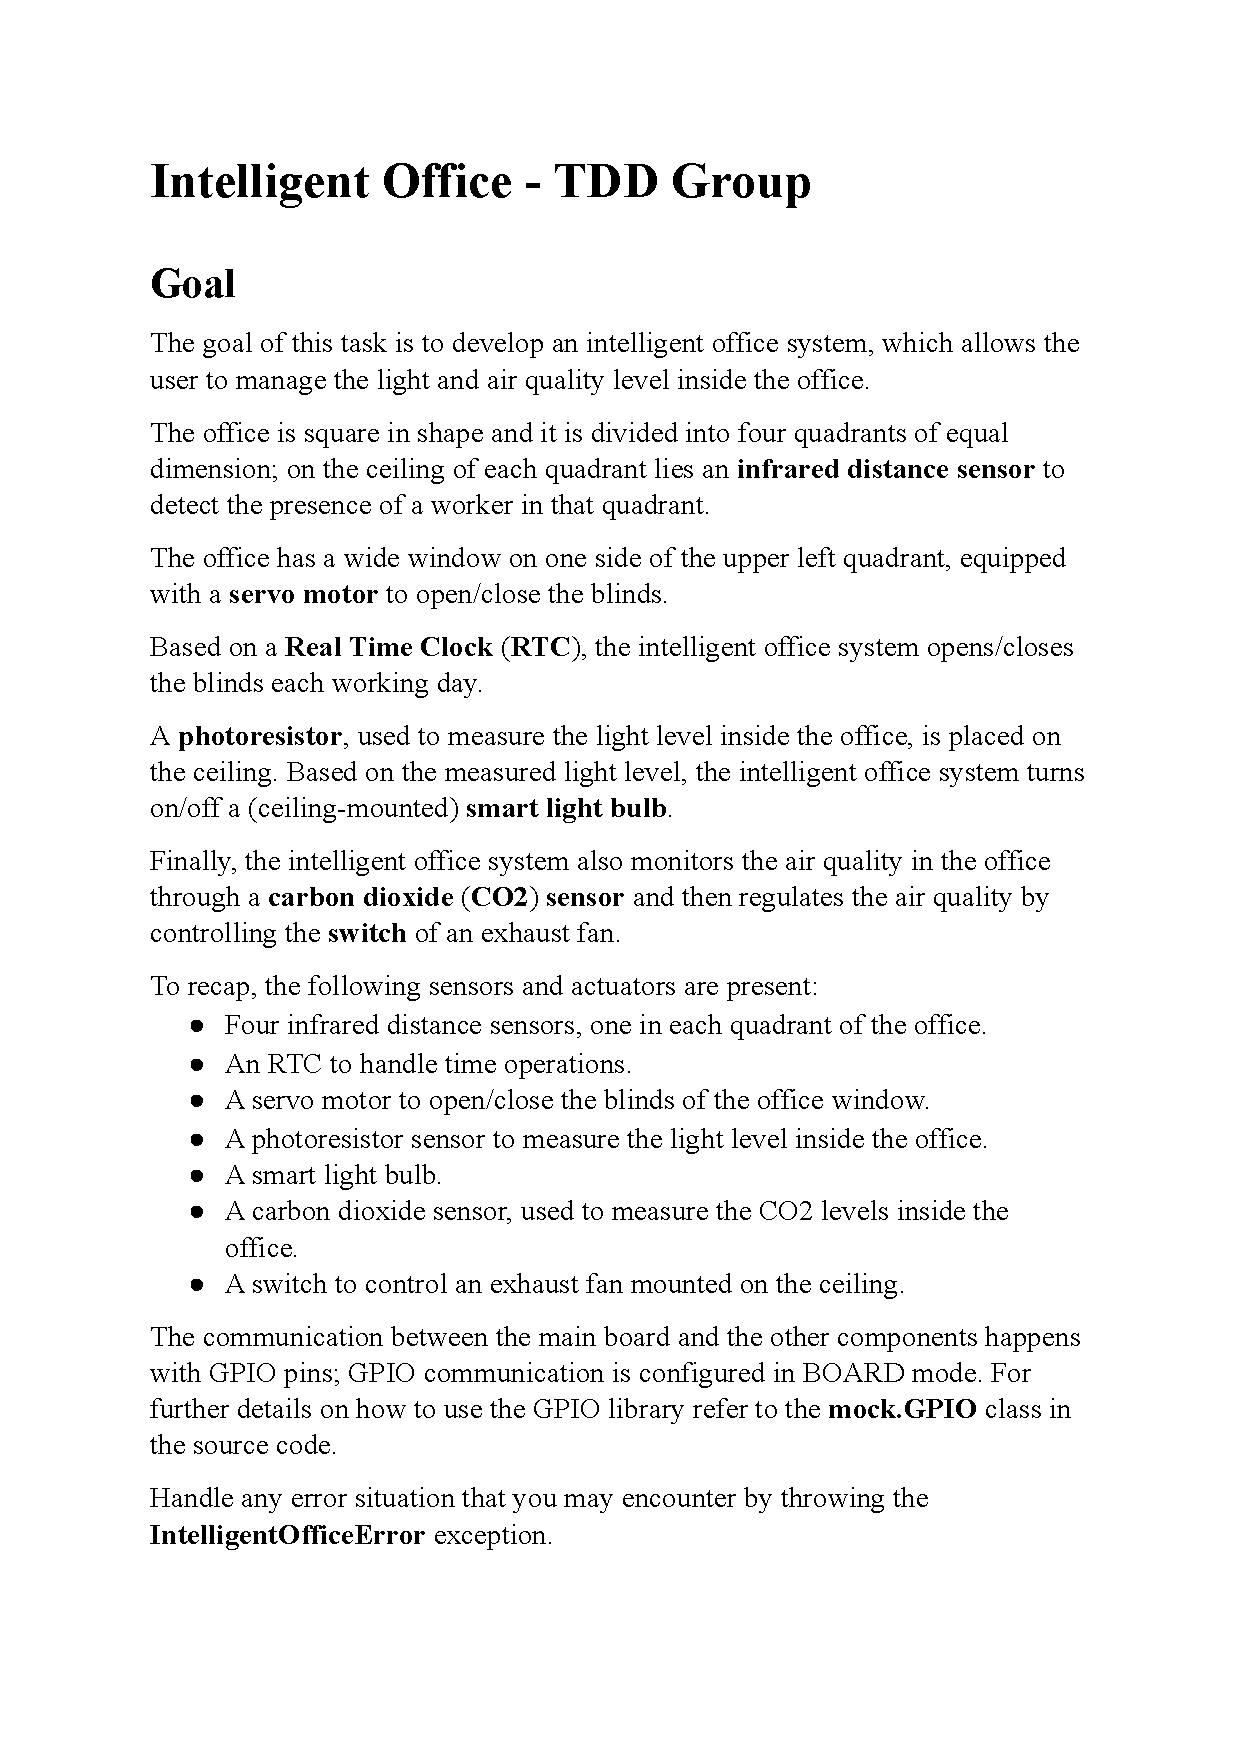
\includepdf[pages=-,scale=.8,pagecommand={},linktodoc=true]{appendix/intelligent_office_tdd.pdf}
    \end{appendices}

\end{document}
